\section{Phase 6}
This is the last phase of the binary bomb. The bomb will greet you with the following lines
{\renewcommand\fcolorbox[4][]{\textcolor{black}{\strut#4}}
\begin{minted}[frame=single,framesep=10pt]{bash}
  [edusc03-052@cheetah022 bomb52]$ ./bomb input.txt
  Welcome to my fiendish little bomb. You have 6 phases with
  which to blow yourself up. Have a nice day!
  Phase 1 defused. How about the next one?
  That's number 2.  Keep going!
  Halfway there!
  So you got that one.  Try this one.
  Good work!  On to the next...
\end{minted}
}\noindent
Again, let's enter a dummy input ``1 2'' into the bomb, and investigate the assembly code. Since the assembly code is too long, I will break it down into different sections.
{\renewcommand\fcolorbox[4][]{\textcolor{cyan}{\strut#4}}
\begin{minted}[frame=single,framesep=10pt]{gas}
  0x0000000000401111 <+0>:     push   %r14
  0x0000000000401113 <+2>:     push   %r13
  0x0000000000401115 <+4>:     push   %r12
  0x0000000000401117 <+6>:     push   %rbp
  0x0000000000401118 <+7>:     push   %rbx
  0x0000000000401119 <+8>:     sub    $0x50,%rsp
  0x000000000040111d <+12>:    lea    0x30(%rsp),%rsi
  0x0000000000401122 <+17>:    callq  0x401473 <read_six_numbers>
  0x0000000000401127 <+22>:    lea    0x30(%rsp),%r12
  0x000000000040112c <+27>:    mov    %r12,%r13
  0x000000000040112f <+30>:    mov    $0x0,%r14d
  0x0000000000401135 <+36>:    jmp    0x40115d <phase_6+76>
  0x0000000000401137 <+38>:    callq  0x401451 <explode_bomb>
\end{minted}
}\noindent
We meet the function \verb+read_six_numbers+ again, which will detonate the bomb if we entered less than 6 integers. Let's reset the bomb and type ``1 2 3 4 5 6'' into the bomb, which will get us pass this first stage of the phase. Next, the bomb load \verb+0x30(%rsp)+ into the register \verb+r12+, let's see what's inside
{\renewcommand\fcolorbox[4][]{\textcolor{black}{\strut#4}}
\begin{minted}[frame=single,framesep=10pt]{bash}
  (gdb) x (0x30+$rsp)
  0x7fffffffe1f0: 0x00000001
\end{minted}
}\noindent
which is our first integer. Then, the bomb will jump to line 76. Let's go to it
{\renewcommand\fcolorbox[4][]{\textcolor{cyan}{\strut#4}}
\begin{minted}[frame=single,framesep=10pt]{gas}
  0x000000000040115d <+76>:    mov    %r13,%rbp
  0x0000000000401160 <+79>:    mov    0x0(%r13),%eax
  0x0000000000401164 <+83>:    sub    $0x1,%eax
  0x0000000000401167 <+86>:    cmp    $0x5,%eax
  0x000000000040116a <+89>:    ja     0x401137 <phase_6+38>
  0x000000000040116c <+91>:    add    $0x1,%r14d
  0x0000000000401170 <+95>:    cmp    $0x6,%r14d
  0x0000000000401174 <+99>:    je     0x40117b <phase_6+106>
  0x0000000000401176 <+101>:   mov    %r14d,%ebx
  0x0000000000401179 <+104>:   jmp    0x401146 <phase_6+53>
\end{minted}
}\noindent
Note that there's two backward jumps, so it might be a loop. After the first two lines, \verb+eax+ is holding our first integer, then, it got decremented and compared with $5$. if it is more than $5$, we jump to the line 38, which is \verb|explode_bomb|, otherwise, we continue with the next lines. Initially, \verb|r14d| is $0$, now it is incremented and compared with $6$, if they are equal, the loop will terminate, otherwise, the bomb assigns the value to \verb|ebx| and continues the loop.
{\renewcommand\fcolorbox[4][]{\textcolor{cyan}{\strut#4}}
\begin{minted}[frame=single,framesep=10pt]{gas}
  0x0000000000401146 <+53>:    movslq %ebx,%rax
  0x0000000000401149 <+56>:    mov    0x30(%rsp,%rax,4),%eax
  0x000000000040114d <+60>:    cmp    %eax,0x0(%rbp)
  0x0000000000401150 <+63>:    jne    0x40113e <phase_6+45>
  0x0000000000401152 <+65>:    callq  0x401451 <explode_bomb>
  0x0000000000401157 <+70>:    jmp    0x40113e <phase_6+45>
  0x0000000000401159 <+72>:    add    $0x4,%r13
\end{minted}
}\noindent
Let's inspect what's residing in \verb|0x30(%rsp,%rax,4)| and \verb|%rbp|
{\renewcommand\fcolorbox[4][]{\textcolor{black}{\strut#4}}
\begin{minted}[frame=single,framesep=10pt]{bash}
  (gdb) x/d $rbp
  0x7fffffffe1f0: 1
  (gdb) x/d $rsp+$rax*4+0x30
  0x7fffffffe1f4: 2
\end{minted}
}\noindent
which is our first and the next number. If they are equal, the bomb will explode, otherwise we go to the line 45
{\renewcommand\fcolorbox[4][]{\textcolor{cyan}{\strut#4}}
\begin{minted}[frame=single,framesep=10pt]{gas}
  0x000000000040113e <+45>:    add    $0x1,%ebx
  0x0000000000401141 <+48>:    cmp    $0x5,%ebx
  0x0000000000401144 <+51>:    jg     0x401159 <phase_6+72>
\end{minted}
}\noindent
Here, \verb|ebx| is incremented and compared with $5$, if it's greater than 5, we go to the line 72, otherwise, continue with the line 53 like above, which continues the loop.\\
This behavior suggest a nested loop, which can be roughly translated into C as
{\renewcommand\fcolorbox[4][]{\textcolor{black}{\strut#4}}
\begin{minted}[frame=single,framesep=10pt]{c}
  // Let's suppose that a[6] = {our 6 numbers}
  int i = 0, j = 0;
  while(i < 6){
    if(a[i] > 6) explode_bomb();
    j = i;
    while(j < 6){
      if(a[i] == a[j]) explode_bomb();
      j++;
    }
    i++;
  }
\end{minted}
}\noindent
In conclusion, this part is for checking whether all the numbers in the input is less than or equal to $6$ and all of them are pairwise distinct, i.e. a permutation from $1$ to $6$. Since our dummy input satisfies this constraint, we can pass this stage.
{\renewcommand\fcolorbox[4][]{\textcolor{cyan}{\strut#4}}
\begin{minted}[frame=single,framesep=10pt]{gas}
  0x000000000040117b <+106>:   lea    0x18(%r12),%rcx
  0x0000000000401180 <+111>:   mov    $0x7,%edx
  0x0000000000401185 <+116>:   mov    %edx,%eax
  0x0000000000401187 <+118>:   sub    (%r12),%eax
  0x000000000040118b <+122>:   mov    %eax,(%r12)
  0x000000000040118f <+126>:   add    $0x4,%r12
  0x0000000000401193 <+130>:   cmp    %r12,%rcx
  0x0000000000401196 <+133>:   jne    0x401185 <phase_6+116>
  0x0000000000401198 <+135>:   mov    $0x0,%esi
  0x000000000040119d <+140>:   jmp    0x4011b8 <phase_6+167>
\end{minted}
}\noindent
This also has a backward jump, so it has a high chance to be
Note that \verb|%r12| is the address of our first number, so \verb|%rcx| is the address that is after our last number.
{\renewcommand\fcolorbox[4][]{\textcolor{black}{\strut#4}}
\begin{minted}[frame=single,framesep=10pt]{bash}
  (gdb) x/8d $r12
  0x7fffffffe1f0: 1       2       3       4
  0x7fffffffe200: 5       6       6306096 0
\end{minted}
}\noindent
Next, \verb|edx| will be equal to \verb|0x7|, and then be assigned to \verb|eax|. Then, \verb|eax| will be subtracted by \verb|r12|, which is our first number, and it will be moved back to \verb|r12|. Finally. \verb|r12| is incremented by $4$, to our second integer. In conlusion, our 6 numbers are modified by the following function
$$ f(x) = 7 - x, $$
where $x$ is our input numbers. After this, our input will become $\{6, 5, 4, 3, 2, 1\}$. Now, let's continue with our bomb.
{\renewcommand\fcolorbox[4][]{\textcolor{cyan}{\strut#4}}
\begin{minted}[frame=single,framesep=10pt]{gas}
  0x00000000004011b8 <+167>:   mov    0x30(%rsp,%rsi,4),%ecx
  0x00000000004011bc <+171>:   mov    $0x1,%eax
  0x00000000004011c1 <+176>:   mov    $0x6032f0,%edx
  0x00000000004011c6 <+181>:   cmp    $0x1,%ecx
  0x00000000004011c9 <+184>:   jg     0x40119f <phase_6+142>
  0x00000000004011cb <+186>:   jmp    0x4011aa <phase_6+153>
\end{minted}
}\noindent
Let's see what's inside the address \verb|0x30(%rsp,%rsi,4)|
{\renewcommand\fcolorbox[4][]{\textcolor{black}{\strut#4}}
\begin{minted}[frame=single,framesep=10pt]{bash}
(gdb) x/8d (0x30+$rsp + $rsi * 4)
0x7fffffffe1f0: 6       5       4       3
0x7fffffffe200: 2       1       6306096 0
\end{minted}
}\noindent
which is our input. This lines of codes can be translated to C as follow
{\renewcommand\fcolorbox[4][]{\textcolor{black}{\strut#4}}
\begin{minted}[frame=single,framesep=10pt]{c}
  // Let a[6] = {our input numbers}
  ecx = a[0];
  eax = 1;
  edx = *0x6032f0;
  if(ecx > 1){
    // Line 142
  } else{
    // Line 153
  }
\end{minted}
}\noindent
Let's inspect \verb|0x6032f0|
{\renewcommand\fcolorbox[4][]{\textcolor{black}{\strut#4}}
\begin{minted}[frame=single,framesep=10pt]{bash}
  (gdb) x 0x6032f0
  0x6032f0 <node1>:       385
\end{minted}
}\noindent
What an interesting name, \verb|node1|. This suggest that it could be some data structures that related to nodes such as linked list, binary tree. Let's examine the address around it
{\renewcommand\fcolorbox[4][]{\textcolor{black}{\strut#4}}
\begin{minted}[frame=single,framesep=10pt]{bash}
  (gdb) x/30x 0x6032f0
  0x6032f0 <node1>: 0x00000181 0x00000001 0x00603300 0x00000000
  0x603300 <node2>: 0x0000010c 0x00000002 0x00603310 0x00000000
  0x603310 <node3>: 0x00000356 0x00000003 0x00603320 0x00000000
  0x603320 <node4>: 0x00000125 0x00000004 0x00603330 0x00000000
  0x603330 <node5>: 0x000003bd 0x00000005 0x00603340 0x00000000
  0x603340 <node6>: 0x000003bb 0x00000006 0x00000000 0x00000000
  0x603350 <bomb_id>: 0x00000034 0x00000000 0x00000000 0x00000000
  0x603360 <host_table>: 0x00402589 0x00000000
\end{minted}
}\noindent
From this, we know that there are $6$ nodes, and each of them as $4$ attributes. However, the last attribute is all $0$, so it does not serve any practical purpose. Hence, there's only $3$ active attributes. The second column is ranging from $1$ to $6$, so it might be the node's id. The third one looks like address values. Further investigation shows that it actually the address of the next node. The below is the diagram of the nodes
\begin{center}
  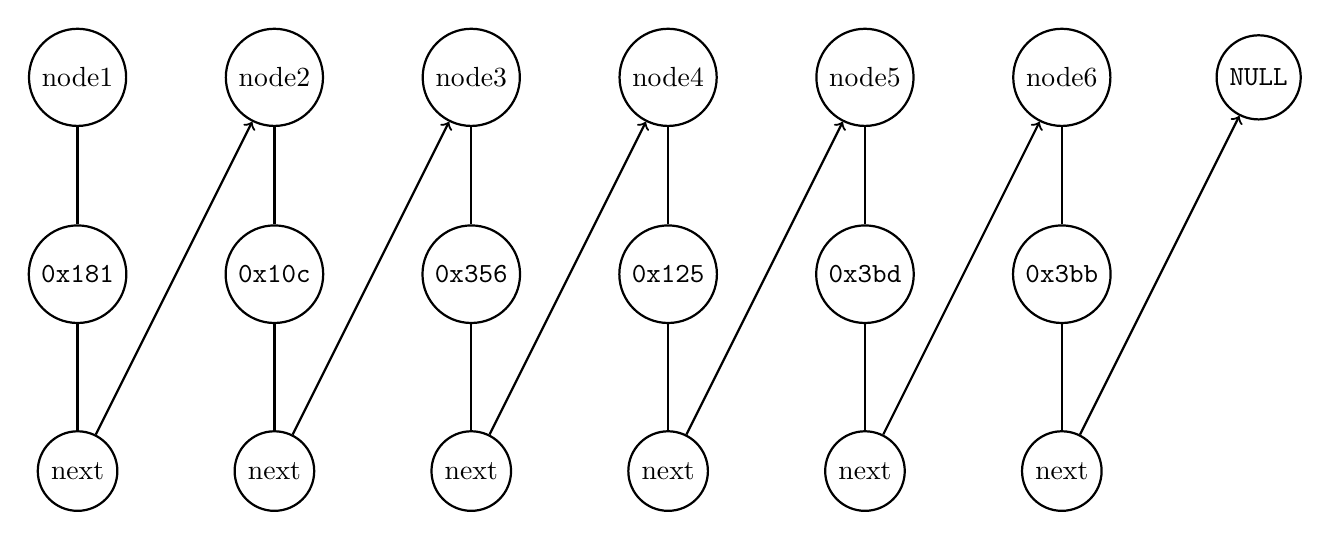
\begin{tikzpicture}[node distance={25mm}, thick, main/.style = {draw, circle}] 
    \node[main] (node1) {node$1$};
    \node[main] (val1) [below of =node1] {\verb|0x181|};
    \node[main] (next1) [below of =val1] {next};
    \node[main] (node2) [right of=node1] {node$2$};
    \node[main] (val2) [below of =node2]  {\verb|0x10c|};
    \node[main] (next2)  [below of =val2]  {next};
    \node[main] (node3) [right of=node2] {node$3$};
    \node[main] (val3) [below of =node3]  {\verb|0x356|};
    \node[main] (next3)  [below of =val3]  {next};
    \node[main] (node4) [right of=node3] {node$4$};
    \node[main] (val4) [below of =node4]  {\verb|0x125|};
    \node[main] (next4)  [below of =val4]  {next};
    \node[main] (node5) [right of=node4] {node$5$};
    \node[main] (val5) [below of =node5]  {\verb|0x3bd|};
    \node[main] (next5)  [below of =val5]  {next};
    \node[main] (node6) [right of=node5] {node$6$};
    \node[main] (val6) [below of =node6]  {\verb|0x3bb|};
    \node[main] (next6)  [below of =val6]  {next};
    \node[main] (null) [right of=node6] {\verb|NULL|};

    \draw (node1) -- (val1);
    \draw (val1) -- (next1);
    \draw[->] (next1) -- (node2);
    \draw (node2) -- (val2);
    \draw (val2) -- (next2);
    \draw[->] (next2) -- (node3);
    \draw (node3) -- (val3);
    \draw (val3) -- (next3);
    \draw[->] (next3) -- (node4);
    \draw (node4) -- (val4);
    \draw (val4) -- (next4);
    \draw[->] (next4) -- (node5);
    \draw (node5) -- (val5);
    \draw (val5) -- (next5);
    \draw[->] (next5) -- (node6);
    \draw (node6) -- (val6);
    \draw (val6) -- (next6);
    \draw[->] (next6) -- (null);
  \end{tikzpicture} 
\end{center}
This suggests the follow definition for a linked list data structure
{\renewcommand\fcolorbox[4][]{\textcolor{black}{\strut#4}}
\begin{minted}[frame=single,framesep=10pt]{c}
  struct node{
    int val, id;
    struct node *link;
  };
\end{minted}
}\noindent
Let's go back to our code, note that there's two backward jumps again, so it must be another loop.
{\renewcommand\fcolorbox[4][]{\textcolor{black}{\strut#4}}
\begin{minted}[frame=single,framesep=10pt]{c}
  if(ecx > 1){
    // Line 142
  }
  // Line 153
\end{minted}
}\noindent
Let's go to the line 142
{\renewcommand\fcolorbox[4][]{\textcolor{cyan}{\strut#4}}
\begin{minted}[frame=single,framesep=10pt]{gas}
  0x000000000040119f <+142>:   mov    0x8(%rdx),%rdx
  0x00000000004011a3 <+146>:   add    $0x1,%eax
  0x00000000004011a6 <+149>:   cmp    %ecx,%eax
  0x00000000004011a8 <+151>:   jne    0x40119f <phase_6+142>
\end{minted}
}\noindent
Let's see that's inside \verb|rdx|
{\renewcommand\fcolorbox[4][]{\textcolor{black}{\strut#4}}
\begin{minted}[frame=single,framesep=10pt]{bash}
  (gdb) x/3 $rdx
  0x6032f0 <node1>: 0x00000181 0x00000001 0x00603300
\end{minted}
}\noindent
which is the first node in our linked list, and \verb|0x8(%rdx)| is the address of the next node, to which we move. Then, \verb|eax| is incremented, and compared with \verb|ecx|, if it is not equal, loop back to the line $142$, if they are equal continue to line $153$. These lines are finding the node in the position specified in our inputs.
{\renewcommand\fcolorbox[4][]{\textcolor{cyan}{\strut#4}}
\begin{minted}[frame=single,framesep=10pt]{gas}
  0x00000000004011aa <+153>:   mov    %rdx,(%rsp,%rsi,8)
  0x00000000004011ae <+157>:   add    $0x1,%rsi
  0x00000000004011b2 <+161>:   cmp    $0x6,%rsi
  0x00000000004011b6 <+165>:   je     0x4011cd <phase_6+188>
\end{minted}
}\noindent
First, it moves the value of our current node into the address \verb|(%rsp,%rsi,8)|, and then increment \verb|rsi|, then continues the loop until $\verb|rsi| = 6$. After the loop is terminated, we go into the line $188$.
{\renewcommand\fcolorbox[4][]{\textcolor{cyan}{\strut#4}}
\begin{minted}[frame=single,framesep=10pt]{gas}
  0x00000000004011cd <+188>:   mov    (%rsp),%rbx
  0x00000000004011d1 <+192>:   mov    0x8(%rsp),%rax
  0x00000000004011d6 <+197>:   mov    %rax,0x8(%rbx)
  0x00000000004011da <+201>:   mov    0x10(%rsp),%rdx
  0x00000000004011df <+206>:   mov    %rdx,0x8(%rax)
  0x00000000004011e3 <+210>:   mov    0x18(%rsp),%rax
  0x00000000004011e8 <+215>:   mov    %rax,0x8(%rdx)
  0x00000000004011ec <+219>:   mov    0x20(%rsp),%rdx
  0x00000000004011f1 <+224>:   mov    %rdx,0x8(%rax)
  0x00000000004011f5 <+228>:   mov    0x28(%rsp),%rax
  0x00000000004011fa <+233>:   mov    %rax,0x8(%rdx)
  0x00000000004011fe <+237>:   movq   $0x0,0x8(%rax)
  0x0000000000401206 <+245>:   mov    $0x5,%ebp
  0x000000000040120b <+250>:   jmp    0x401216 <phase_6+261>
\end{minted}
}\noindent
Note that \verb|rsp| here is holding our values of the linked list. Let's inspect them, using the following custom function in \verb|gdb|.
{\renewcommand\fcolorbox[4][]{\textcolor{black}{\strut#4}}
\begin{minted}[frame=single,framesep=10pt]{bash}
  define pa
    set var $i = 1
    while $i <= 6
      printf "a[%d] = %x\n", $i, **(int*)($arg0 + 0x8*($i-1))
      set var $i = $i + 1
    end
  end
\end{minted}
}\noindent
Using this custom command with an argument of \verb|rsp|, we obtain the following
{\renewcommand\fcolorbox[4][]{\textcolor{black}{\strut#4}}
\begin{minted}[frame=single,framesep=10pt]{bash}
  (gdb) pa $rsp
  a[1] = 0x3bb
  a[2] = 0x3bd
  a[3] = 0x125
  a[4] = 0x356
  a[5] = 0x10c
  a[6] = 0x181
\end{minted}
}\noindent
The value now is shuffled according to our modified input, i.e. ``6 5 4 3 2 1''. Meaning, the first value is the value of \verb|node6|, the second value is the value of \verb|node5|, and so on. These lines just move all the data from \verb|rsp| to \verb|rbx|. Now, let's see the last few lines
{\renewcommand\fcolorbox[4][]{\textcolor{cyan}{\strut#4}}
\begin{minted}[frame=single,framesep=10pt]{gas}
  0x000000000040120b <+250>:   jmp    0x401216 <phase_6+261>
  0x000000000040120d <+252>:   mov    0x8(%rbx),%rbx
  0x0000000000401211 <+256>:   sub    $0x1,%ebp
  0x0000000000401214 <+259>:   je     0x401227 <phase_6+278>
  0x0000000000401216 <+261>:   mov    0x8(%rbx),%rax
  0x000000000040121a <+265>:   mov    (%rax),%eax
  0x000000000040121c <+267>:   cmp    %eax,(%rbx)
  0x000000000040121e <+269>:   jge    0x40120d <phase_6+252>
  0x0000000000401220 <+271>:   callq  0x401451 <explode_bomb>
  0x0000000000401225 <+276>:   jmp    0x40120d <phase_6+252>
\end{minted}
}\noindent
Firstly, we start at the line 261. Here, \verb|eax| is holding our second value, i.e. \verb|a[2]|. Then, the bomb compares \verb|a[1]| and \verb|a[2]|, if $a[1] \geq a[2]$ then we continue with our loop, otherwise, the bomb will explode. In the next iterations, the bomb also compares the current value with the next value, i.e. it is checking whether $a[i] \geq a[i + 1]$, if there exists an $i$ that violates the condition, the bomb will detonate, otherwise, it jumps peacefully to the line 278, which is the end of our function.
{\renewcommand\fcolorbox[4][]{\textcolor{cyan}{\strut#4}}
\begin{minted}[frame=single,framesep=10pt]{gas}
  0x0000000000401227 <+278>:   add    $0x50,%rsp
  0x000000000040122b <+282>:   pop    %rbx
  0x000000000040122c <+283>:   pop    %rbp
  0x000000000040122d <+284>:   pop    %r12
  0x000000000040122f <+286>:   pop    %r13
  0x0000000000401231 <+288>:   pop    %r14
  0x0000000000401233 <+290>:   retq
\end{minted}
}\noindent
In conclusion, the last few lines are checking if our values from the array ``\verb|a|'' is nonincreasing. If it is, then we defuse the bomb, otherwise, the bomb will detonate. In our case of dummy input, the bomb will detonate after it detects $a[1] < a[2]$, which violates the condition. Therefore, we have to find a permutation of $\{1, 2, 3, 4, 5, 6\}$ so that our final ``array'' is nonincreasing. Recall that the original values of the nodes are
\begin{center}
  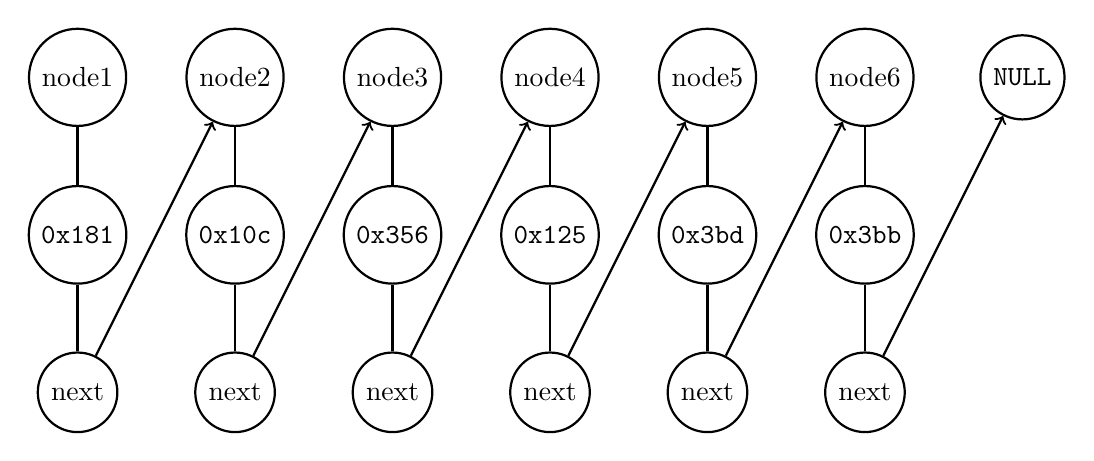
\begin{tikzpicture}[node distance={20mm}, thick, main/.style = {draw, circle}] 
    \node[main] (node1) {node$1$};
    \node[main] (val1) [below of =node1] {\verb|0x181|};
    \node[main] (next1) [below of =val1] {next};
    \node[main] (node2) [right of=node1] {node$2$};
    \node[main] (val2) [below of =node2]  {\verb|0x10c|};
    \node[main] (next2)  [below of =val2]  {next};
    \node[main] (node3) [right of=node2] {node$3$};
    \node[main] (val3) [below of =node3]  {\verb|0x356|};
    \node[main] (next3)  [below of =val3]  {next};
    \node[main] (node4) [right of=node3] {node$4$};
    \node[main] (val4) [below of =node4]  {\verb|0x125|};
    \node[main] (next4)  [below of =val4]  {next};
    \node[main] (node5) [right of=node4] {node$5$};
    \node[main] (val5) [below of =node5]  {\verb|0x3bd|};
    \node[main] (next5)  [below of =val5]  {next};
    \node[main] (node6) [right of=node5] {node$6$};
    \node[main] (val6) [below of =node6]  {\verb|0x3bb|};
    \node[main] (next6)  [below of =val6]  {next};
    \node[main] (null) [right of=node6] {\verb|NULL|};

    \draw (node1) -- (val1);
    \draw (val1) -- (next1);
    \draw[->] (next1) -- (node2);
    \draw (node2) -- (val2);
    \draw (val2) -- (next2);
    \draw[->] (next2) -- (node3);
    \draw (node3) -- (val3);
    \draw (val3) -- (next3);
    \draw[->] (next3) -- (node4);
    \draw (node4) -- (val4);
    \draw (val4) -- (next4);
    \draw[->] (next4) -- (node5);
    \draw (node5) -- (val5);
    \draw (val5) -- (next5);
    \draw[->] (next5) -- (node6);
    \draw (node6) -- (val6);
    \draw (val6) -- (next6);
    \draw[->] (next6) -- (null);
  \end{tikzpicture} 
\end{center}
After sorting, the nodes will be in the following order
\begin{center}
  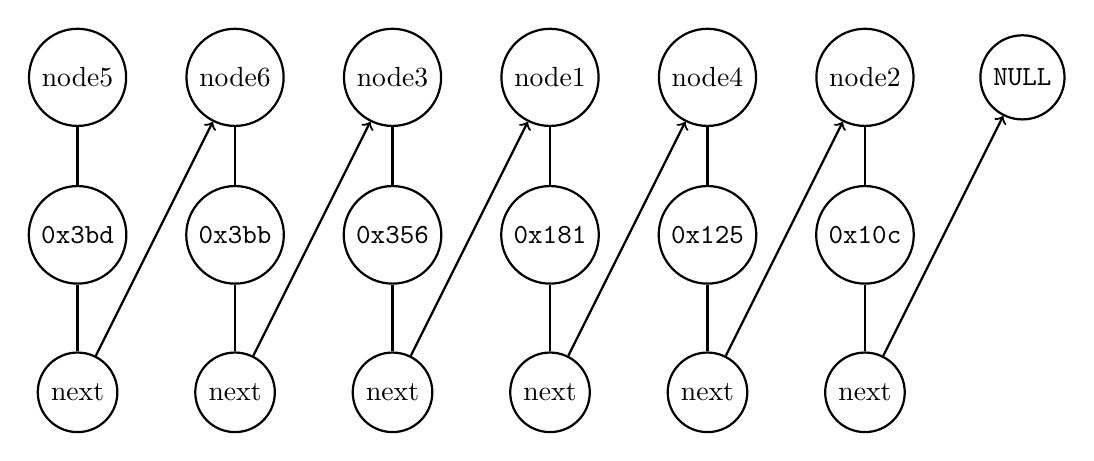
\begin{tikzpicture}[node distance={20mm}, thick, main/.style = {draw, circle}] 
    \node[main] (node1) {node$5$};
    \node[main] (val1) [below of =node1] {\verb|0x3bd|};
    \node[main] (next1) [below of =val1] {next};
    \node[main] (node2) [right of=node1] {node$6$};
    \node[main] (val2) [below of =node2]  {\verb|0x3bb|};
    \node[main] (next2)  [below of =val2]  {next};
    \node[main] (node3) [right of=node2] {node$3$};
    \node[main] (val3) [below of =node3]  {\verb|0x356|};
    \node[main] (next3)  [below of =val3]  {next};
    \node[main] (node4) [right of=node3] {node$1$};
    \node[main] (val4) [below of =node4]  {\verb|0x181|};
    \node[main] (next4)  [below of =val4]  {next};
    \node[main] (node5) [right of=node4] {node$4$};
    \node[main] (val5) [below of =node5]  {\verb|0x125|};
    \node[main] (next5)  [below of =val5]  {next};
    \node[main] (node6) [right of=node5] {node$2$};
    \node[main] (val6) [below of =node6]  {\verb|0x10c|};
    \node[main] (next6)  [below of =val6]  {next};
    \node[main] (null) [right of=node6] {\verb|NULL|};

    \draw (node1) -- (val1);
    \draw (val1) -- (next1);
    \draw[->] (next1) -- (node2);
    \draw (node2) -- (val2);
    \draw (val2) -- (next2);
    \draw[->] (next2) -- (node3);
    \draw (node3) -- (val3);
    \draw (val3) -- (next3);
    \draw[->] (next3) -- (node4);
    \draw (node4) -- (val4);
    \draw (val4) -- (next4);
    \draw[->] (next4) -- (node5);
    \draw (node5) -- (val5);
    \draw (val5) -- (next5);
    \draw[->] (next5) -- (node6);
    \draw (node6) -- (val6);
    \draw (val6) -- (next6);
    \draw[->] (next6) -- (null);
  \end{tikzpicture} 
\end{center}
Thus, the correct permutation should be $\{5, 6, 3, 1, 4, 2\}$.However, note that before shuffling the linked list, our input is modified by the function
$$ f(x) = 7 - x $$
Therefore, the correct input should be ``\verb|2 1 4 6 3 5|''. Resetting the bomb and typing in the correct string, we have successfully defused the entire bomb!
{\renewcommand\fcolorbox[4][]{\textcolor{black}{\strut#4}}
\begin{minted}[frame=single,framesep=10pt]{text}
  [edusc03-052@cheetah022 bomb52]$ ./bomb input.txt
  Welcome to my fiendish little bomb. You have 6 phases with
  which to blow yourself up. Have a nice day!
  Phase 1 defused. How about the next one?
  That's number 2.  Keep going!
  Halfway there!
  So you got that one.  Try this one.
  Good work!  On to the next...
  2 1 4 6 3 5
  Congratulations! You've defused the bomb!
\end{minted}
}\noindent



\newpage